%!TEX root = ../master_thesis.tex
\chapter{Evaluation and Discussion}
\label{ch:results}

\section{Evaluation Setup}
\label{sec:res}


\subsection{Speaker Detection Network}
\label{subsec:sdn}
\begin{table}[]
    \centering
    \begin{tabular}{c|cc}
    \toprule
    \textbf{Method} & \multicolumn{2}{c}{\textbf{Accuracy}}\\
    & Held-out & New Speakers \\
    \midrule
        TDNN &  &\\
        TDNN-Attn. & &\\
    \end{tabular}
    \caption{Evaluation of Speaker Detection System}
    \label{tab:data_stat}
\end{table}

\subsection{Evaluation Metric}
\label{subsec:eval_metrics}
Speaker detection system on training set of Librispeech. 
Evaluation on held out set.
\subsubsection{Inception Score}
\label{subsec:inception_score}
On $30\%$ held out samples of $251$ speakers the $\text{IS}=29.51\pm 0.37$. 
\subsubsection{Fr\'{e}chet Inception Distance}


\begin{figure}[h]
\centering
\subfloat[Magnitude Spectrogram]{
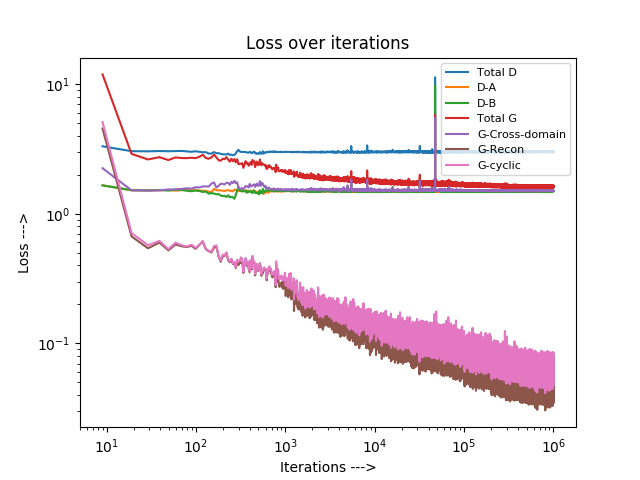
\includegraphics[width=0.4\textwidth]{master_thesis_template/figs/vc-gan/mag_vc_plot.png}
\label{fig:mag_spect}}
\qquad
\subfloat[Log Magnitude Spectrogram]{
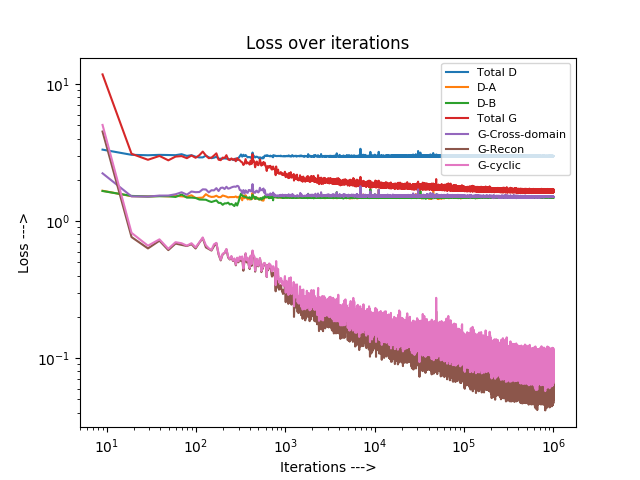
\includegraphics[width=0.4\textwidth]{master_thesis_template/figs/vc-gan/logmag_loss_plot.png}
\label{fig:logmag_spect}}
\subfloat[Mel Spectrogram]{
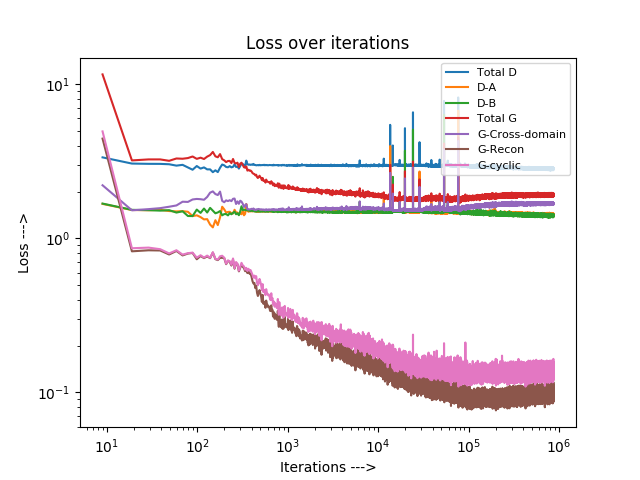
\includegraphics[width=0.4\textwidth]{master_thesis_template/figs/vc-gan/mel_loss_plot.png}
\label{fig:mel_spect}}
\qquad
\subfloat[Log Mel Spectrogram]{
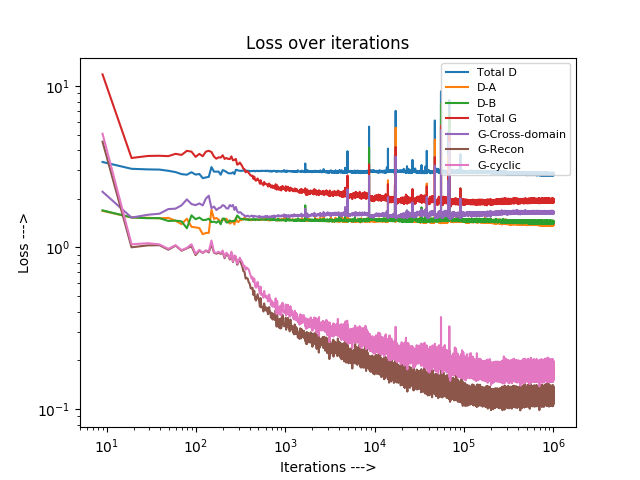
\includegraphics[width=0.4\textwidth]{master_thesis_template/figs/vc-gan/log_mel_loss_plot.png}
\label{fig:logmel_spect}}
\caption{Plot of loss function for different representation of signal. The $x$ axis is on the log scale}
\label{fig:vc-gan-loss}
\end{figure}




\subsubsection{Domain Classifier}
\label{subsub:dclf}
\subsection{Ablation Study}

\section{Discussion}
\label{sec:discussion}



\begin{table}
    \centering
    \begin{tabular}{cccccc}
    \toprule
    \textbf{Method}     & \textbf{Spectrogram} & \textbf{IS} & \textbf{FID} & \multicolumn{2}{c}{\textbf{Accuracy}}\\
    \cmidrule(r){5-6}
    & & & & \textbf{Test}|&|\textbf{Gen.}\\
    \midrule
     VC-GAN    & Mag & & & \\
         & Mel & & &\\
         & Log-Mag && & \\
         & Log-Mel & & &\\
    \midrule
     VC-Con-GAN    & Mag & & & \\
%         & Mel & & &\\
         & Log-Mag & $19.49\pm0.50$ & 28.56 & \\
%         & Log-Mel & & &\\  
    \midrule
     VC-GAN    & Mag-IF & & & \\
         & Log-Mag-IF& & &\\ 
    \midrule
     VC-Con-GAN    & Mag-IF & & & \\
         & Log-Mag-IF& & &\\ 
    \midrule
     VC-Con-GL-GAN    & Mag-IF& & & \\
%         & Mel-IF& & &\\
         & Log-Mag-IF& & & \\
%         & Log-Mel & & &\\          
    \midrule
     VC-Con-GAN-multiD    & Mag-IF & & & \\
         & Log-Mag-IF& & &\\               
    \bottomrule 
    \end{tabular}
    \caption{Evaluation of generated samples of different spectrogram representation. We compare Inception Score (IS), Fr\'{e}chet Distance(FID) and domain detection accuracy. We report accuracy on unseen original test samples and generated samples.}
    \label{tab:eval_gan}
\end{table}


\begin{table}
    \centering
    \scriptsize
    \begin{tabular}{ccccccc}
    \toprule
    \textbf{Method} & \textbf{Spectrogram} &\textbf{All Loss terms} & \textbf{No SpecCon} & \textbf{No VAE} & \textbf{No CC} &\textbf{No CC+VAE}\\
    \midrule
     VC-GAN    & Mag & & & & \\
         & Mel & &  & &\\
         & Log-Mag & & & & \\
         & Log-Mel & & & &\\
    \bottomrule 
    \end{tabular}
    \caption{In this part we compare the effect of different loss terms.}
    \label{tab:ablation_study}
\end{table}

